\documentclass{article}
\usepackage{listings}
\usepackage{hyperref}
\usepackage{fancybox}
\usepackage{graphicx}
\author{Fedor Baart}
\title{Improving hyrax performance for small data requests}
\begin{document}
\maketitle
\begin{abstract}
  Testing the performance of the hyrax opendap server showed a latency for small requests. This report describes possibilities to improve the performance of hyrax for small requests. 
\end{abstract}
\section{Introduction}
After using the hyrax server from existing code which was doing a lot of small (arrays of size $1 \times 800$) requests a lower than expected performance was noted. 

\section{Tests}
\subsection{Test system}
A test system was setup in a virtual machine on the following hard \& software
\begin{itemize}
\item{host} iMac 2.4Ghz Intel Core 2 Duo, 2GB, OSX 10.5.5
\item{virtual machine} 1 processor, 512MB, Ubuntu 8.10, running under vmware fusion
\item{servlet container} tomcat 6.0.18 (binary download, running under user folder)
\item{hyrax} bes, dap\_server, libdap, hdf5\_handler, freeform\_handler, netcdf\_handler   all at revision 20022 from the trunk 
\item{hdf} hdf5-1.8.2
\item{netcdf} netcdf-4.0
\item{wireshark} 1.0.3
\end{itemize}
\subsection{Test script}
To test the performance the script displayed in listing \ref{lis:perf} was used. 
\lstinputlisting[frame=shadowbox,frameround=tttt,flexiblecolumns=true,caption=Performance measurements,breaklines=true,label=lis:perf,language=bash]{testperformance.sh}
Detailed analysis was done using the statistics from wireshark listening on the loopback interface. 
\section{Results}
The conversation between curl and tomcat is listed in listing \ref{lis:curl-tomcat}.
\lstinputlisting[frame=shadowbox,frameround=tttt,flexiblecolumns=true,breaklines=true,caption=Conversation between ,label=lis:curl-tomcat]{pre/httpconversation.txt}
The total response time for this request is $0.40065$ seconds with a standard deviation of $0.0086$ seconds. 

Next we look at the conversation between the BES and the olfs. The conversation is listed in listing \ref{lis:bes-olfs}.
\lstinputlisting[frame=shadowbox,frameround=tttt,flexiblecolumns=true,breaklines=true,caption=Conversation between ,label=lis:bes-olfs,language=xml]{pre/besconversation.txt}
The time for each timing can be seen in the roundtrip time graph in figure \ref{fig:roundtrip}
\begin{figure}
\centering
\includegraphics[width=8cm]{pre/roundtriptime}
\caption{Roundtrip Time for bes-olfs communication}\label{fig:roundtrip}
\end{figure}
The long round trips are the time it takes to respond between the \textit{000011ad} and the start of the xml response. 

\section{Analysis}
A response time of $0.4$ seconds for any request is higher than needed. If we look at where the $0.4$ seconds is spent we can see that the communication between bes and olfs is repetitive. The request showinfo is repeated 4 times before the data request is sent to the bes. Approximately $0.04 \times 4$ seconds are spend on replying to the same showinfo request. 

The $0.04$ seconds can be reduced by profiling the bes and dap-server application. The number of requests currently 4 can be reduced by adapting the olfs application. We'll try to decrease the number of requests send from olfs to bes. 

The showinfo request originates from the call in the file BesXmlApi as can be seen in listing \ref{lis:besxmlapi}
\lstinputlisting[frame=shadowbox,frameround=tttt,numbers=left,stepnumber=5,numberstyle=\tiny,flexiblecolumns=true,caption=BesXmlApi.java,breaklines=true,label=lis:besxmlapi,language=java,firstline=538,lastline=550]{pre/BesXmlAPI.java}

This is called by the constructor of BESDataSource 

\lstinputlisting[frame=shadowbox,frameround=tttt,frame=shadowbox,frameround=tttt,numbers=left,stepnumber=5,numberstyle=\tiny,flexiblecolumns=true,caption=BESDataSource.java,breaklines=true,label=lis:besdatasource,language=java,firstline=72,lastline=82]{pre/BESDataSource.java}

The BESDataSource is constructed by the DapDispatchHandler

\lstinputlisting[frame=shadowbox,frameround=tttt,numbers=left,stepnumber=5,numberstyle=\tiny,flexiblecolumns=true,caption=BESDataSource.java,breaklines=true,label=lis:dapdispatchhandler,language=java,firstline=270,lastline=273]{pre/DapDispatchHandler.java}



\section{Suggested improvement}
To limit the number of times the showinfo request is sent we can limit the number of times the BESDataSource is constructed. This can be done using memoization \footnote{\url{http://en.wikipedia.org/wiki/Memoization}}. It can be implemented using a hash table as shown in listing \ref{lis:diff}. 
\lstinputlisting[frame=shadowbox,frameround=tttt,flexiblecolumns=true,caption=Using a hash table to cache BESDataSource objects,breaklines=true,label=lis:diff,language=java]{besdatasourcecache.diff}

There's probably a more java based way to do this, maybe using annotations or closures.  

\section{Testing}
The performance test script as listed in listing \ref{lis:perf} is again used to test the performance after the application of the changes listed in the previous section. The measurements of the response times are significantly lower with an average of $0.045$ seconds and a standard deviation of $0.00339$. The measurements of both pre and post patch response times are shown in figure \ref{fig:response}. 

\begin{figure*}
\centering
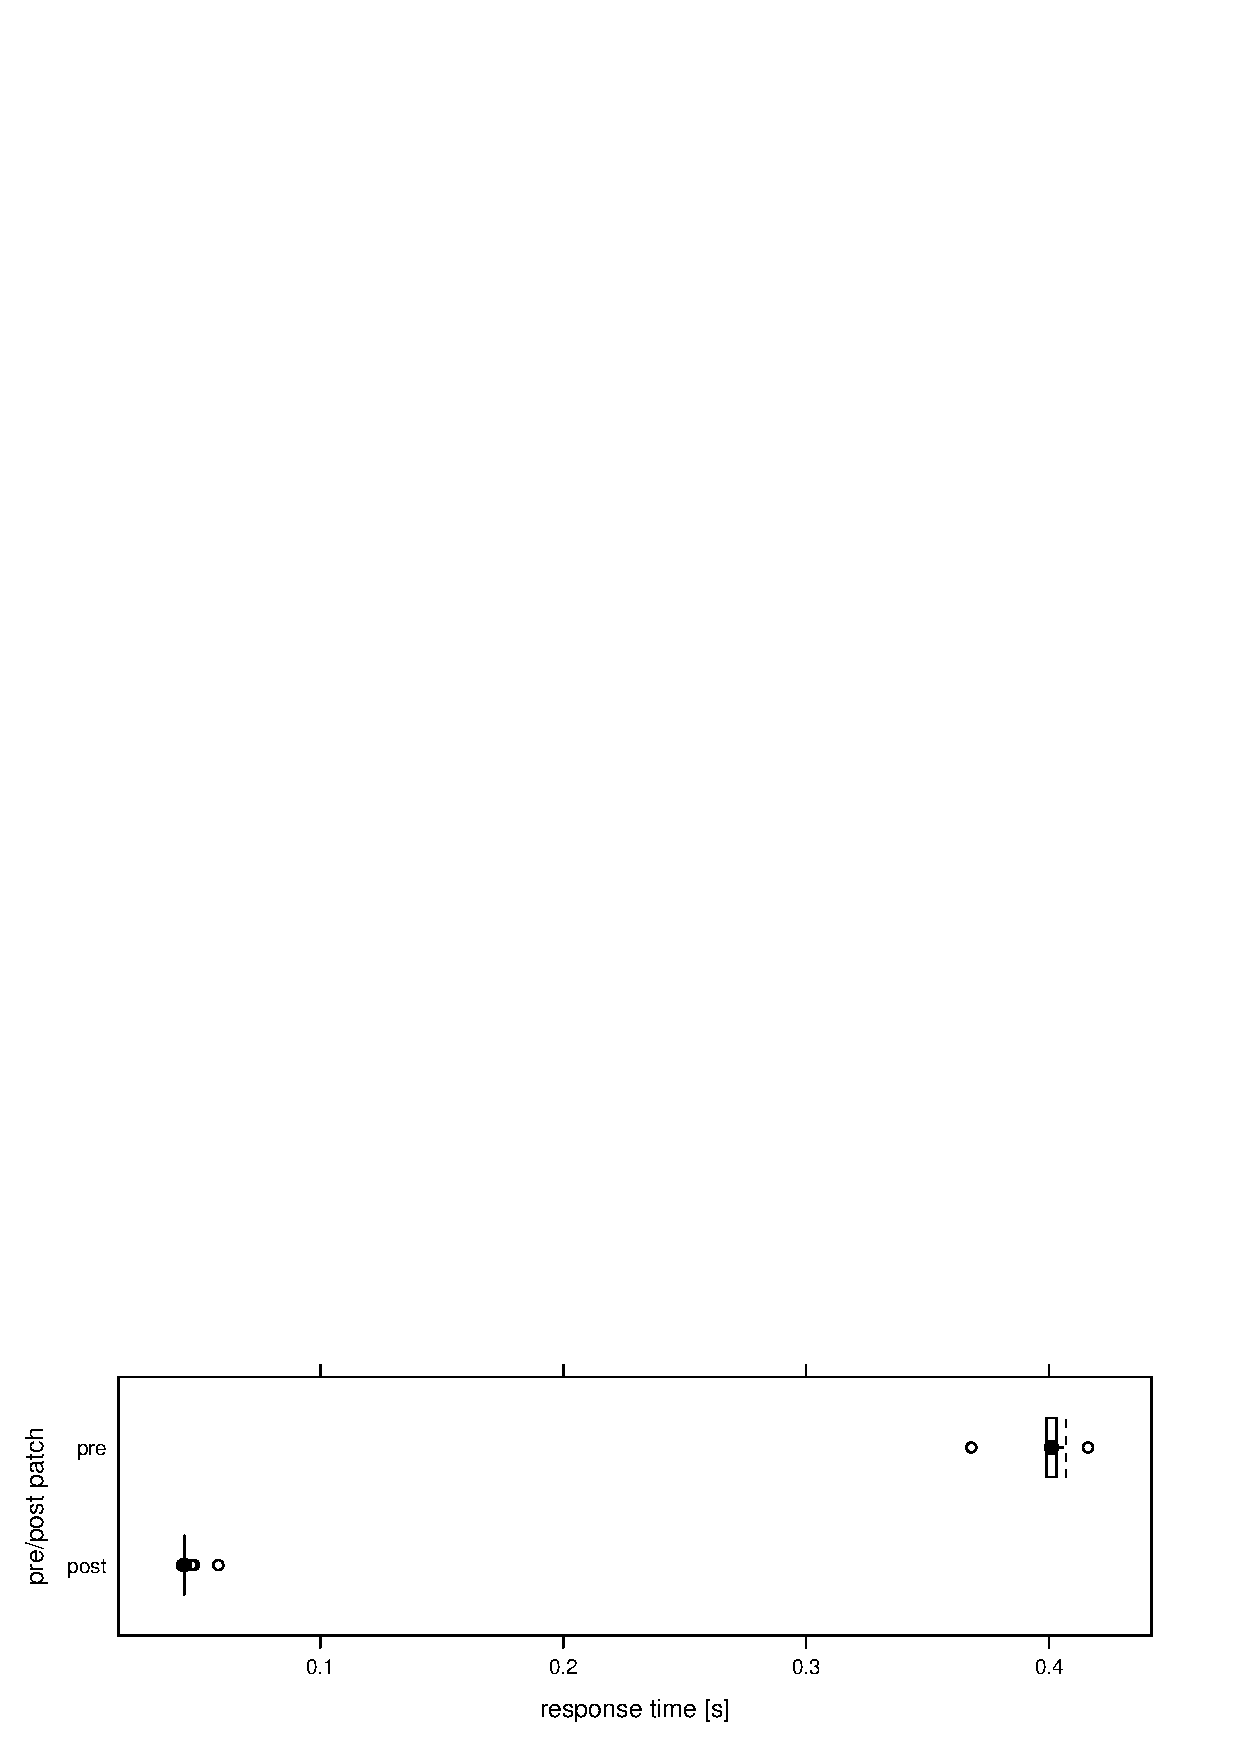
\includegraphics[width=8cm,height=3cm]{prepost}
\caption{Response times for ascii web request (lower is better)}
\label{fig:response}
\end{figure*}

\section{Analysis}
By caching the creation of BESDataSource onlybjects a speed increase of up to a factor $8.9$ can be reached. This only applies to small requests. Also the first time a BESDataSource is accessed by a thread from the olfs the response will be twice as long because the data source is read and the BESDataSource object is created. Resulting in a speed increase of only $4.5$. 

A possible caveat is that if a BESDataSource object is cached and data is changed or removed on disk this might lead to unexpected behaviour using this approach. 

Another thing to look at is the ammount the memory footprint increases by caching the BESDataSource objects.

The speed of small requests can further be improved by limiting the $0.04$ seconds it takes for the bes to respond to a request. This can be done using by profiling the bes, libdap and dap-server applications. 
\end{document}

